%!TEX program = xelatex
%!TEX spellcheck = en_GB
\documentclass[final]{article}
% Include all project wide packages here.
%\usepackage{fullpage}
\usepackage[a4paper,margin=2.5cm,top=2cm]{geometry}
\usepackage{polyglossia}
\setmainlanguage{english}
\usepackage{csquotes}
\usepackage{graphicx}
\usepackage{pdfpages}
\usepackage{caption}
\usepackage[list=true]{subcaption}
\usepackage{float}
\usepackage{standalone}
\usepackage{import}
\usepackage{tocloft}
\usepackage{wrapfig}
\usepackage{authblk}
\usepackage{array}
\usepackage{booktabs}
\usepackage[title,titletoc]{appendix}
\usepackage{fontspec}
\usepackage{pgfplots}
\usepackage{tikz}
\usepackage{tikz-uml}
\usepackage{siunitx}
\usepackage{units}
\usepackage{amsmath}
\usepackage{mathtools}
\usepackage{unicode-math}
\usepackage{rotating}
\usepackage{titlesec}
\usepackage{titletoc}
\usepackage{blindtext}
\usepackage{color}
\usepackage{enumitem}
\usepackage{tabularx}
\usepackage{titling}
\usepackage[%
siunitx,
fulldiodes,
europeanvoltages,
europeancurrents,
europeanresistors,
americaninductors,
smartlabels]{circuitikz}

\newcommand{\matlab}{{\textsc{matlab }}}

\usetikzlibrary{calc}
\usetikzlibrary{positioning}
\usetikzlibrary{automata}
\usetikzlibrary{arrows.meta}

\tikzstyle{every state}=[fill=tu-cyan,align=center,draw=black,line width=1pt,node distance=3cm,minimum width = 1.8cm]%for FSMs casper
\tikzstyle{every initial by arrow}=[initial text={Reset}]
\newcommand{\setpathasarrows}{\tikzstyle{every path}=[auto,line width=1.5pt,line cap=round,line join=round]}

\pgfplotsset{compat=newest}
\pgfplotsset{plot coordinates/math parser=false}
\usetikzlibrary{plotmarks}
\usepgfplotslibrary{patchplots}
\newlength\figureheight
\newlength\figurewidth

\tikzset{every axis/.style={xticklabel style={align=right}}}

\usepackage[
%backend=bibtex,
backend=biber,
	texencoding=utf8,
bibencoding=utf8,
style=numeric,
citestyle=numeric,
    sortlocale=en_US,
    language=auto,
    backref=true,
    abbreviate=false,
    date=iso8601
]{biblatex}


\usepackage{listings}
\newcommand{\includecode}[4][c]{\lstinputlisting[caption=#2, escapechar=, style=#1,label=#4]{#3}}
\newcommand{\superscript}[1]{\ensuremath{^{\textrm{#1}}}}
\newcommand{\subscript}[1]{\ensuremath{_{\textrm{#1}}}}


\newcommand{\chapternumber}{\thechapter}
\renewcommand{\appendixname}{Appendix}
\renewcommand{\appendixtocname}{Appendices}
\renewcommand{\appendixpagename}{Appendices}


\setlist[enumerate]{labelsep=*, leftmargin=1.5pc}
\setlist[enumerate,1]{label=\arabic*., ref=\arabic*}
\setlist[enumerate,2]{label=\arabic*.,ref=\theenumi.\arabic*}
\setlist[enumerate,3]{label=\arabic*., ref=\theenumii.\arabic*}

\setcounter{chapter}{-1} %start chapter numbers with 0

\usepackage{xr-hyper}
\usepackage[hidelinks]{hyperref} %<--------ALTIJD ALS LAATSTE
\usepackage[nameinlink,noabbrev,capitalise]{cleveref} %<------- Clever Ref moet na hyperref
\crefname{app}{Appendix}{Appendices}
%\renewcommand{\familydefault}{\sfdefault}


\setmainfont{Myriad Pro}[Ligatures={Common,TeX}]
%\setmathfont{Asana Math}
\setmathfont{Asana-Math.otf}
\setmonofont[Scale=0.9]{Lucida Console}
\newfontfamily\headingfont{Minion Pro}[Ligatures={Common,TeX}]


%Design colors
\definecolor{accent1}{RGB}{0,100,200}
\definecolor{accent2}{RGB}{0,50,100}
\definecolor{tu-cyan}{RGB}{0,166,214}

\newcommand{\hsp}{\hspace{20pt}}
% \titleformat{\chapter}[hang]{\Huge\headingfont}{\chapternumber\hsp\textcolor{accent2}{|}\hsp}{0pt}{\Huge\headingfont}

% \titleformat{name=\chapter,numberless}[hang]{\Huge\headingfont}{\hsp\textcolor{accent2}{|}\hsp}{0pt}{\Huge\headingfont}

% \titleformat{\section}[block]{\LARGE\headingfont}{\arabic{chapter}.\arabic{section}}{0.4em}{}
% \titleformat{\subsection}[block]{\Large\headingfont}{\arabic{chapter}.\arabic{section}.\arabic{subsection}}{0.4em}{}
% \titleformat{\subsubsection}[block]{\large\headingfont}{\arabic{chapter}.\arabic{section}.\arabic{subsection}.\arabic{subsubsection}}{0.4em}{}
\renewcommand{\arraystretch}{1.2}
\renewcommand{\baselinestretch}{1.25} 

\renewcommand\cfttoctitlefont{\headingfont\Huge}
\renewcommand\cftloftitlefont{\headingfont\Huge}
\renewcommand\cftlottitlefont{\headingfont\Huge}
\setcounter{lofdepth}{2}
\setcounter{lotdepth}{2}


\setlength{\parindent}{0pt}
\setlength{\parskip}{1em}


%SIuntix settings:
%default: 0V to 10V
%custom: 0 - 10V
\sisetup{range-phrase=--}
\sisetup{range-units=single}
\DeclareSIUnit\years{years}

%For code listings
\definecolor{black}{rgb}{0,0,0}
\definecolor{browntags}{rgb}{0.65,0.1,0.1}
\definecolor{bluestrings}{rgb}{0,0,1}
\definecolor{graycomments}{rgb}{0.4,0.4,0.4}
\definecolor{redkeywords}{rgb}{1,0,0}
\definecolor{bluekeywords}{rgb}{0.13,0.13,0.8}
\definecolor{greencomments}{rgb}{0,0.5,0}
\definecolor{redstrings}{rgb}{0.9,0,0}
\definecolor{purpleidentifiers}{rgb}{0.01,0,0.01}


\lstdefinestyle{csharp}{
language=[Sharp]C,
showspaces=false,
showtabs=false,
breaklines=true,
showstringspaces=false,
breakatwhitespace=true,
escapeinside={(*@}{@*)},
columns=fullflexible,
commentstyle=\color{greencomments},
keywordstyle=\color{bluekeywords}\bfseries,
stringstyle=\color{redstrings},
identifierstyle=\color{purpleidentifiers},
basicstyle=\ttfamily\small}

\lstdefinestyle{c}{
language=C,
showspaces=false,
showtabs=false,
breaklines=true,
showstringspaces=false,
breakatwhitespace=true,
escapeinside={(*@}{@*)},
columns=fullflexible,
commentstyle=\color{greencomments},
keywordstyle=\color{bluekeywords}\bfseries,
stringstyle=\color{redstrings},
identifierstyle=\color{purpleidentifiers},
}

\lstdefinestyle{matlab}{
language=Matlab,
showspaces=false,
showtabs=false,
breaklines=true,
showstringspaces=false,
breakatwhitespace=true,
escapeinside={(*@}{@*)},
columns=fullflexible,
commentstyle=\color{greencomments},
keywordstyle=\color{bluekeywords}\bfseries,
stringstyle=\color{redstrings},
identifierstyle=\color{purpleidentifiers}
}

\lstdefinestyle{vhdl}{
language=VHDL,
showspaces=false,
showtabs=false,
breaklines=true,
showstringspaces=false,
breakatwhitespace=true,
escapeinside={(*@}{@*)},
columns=fullflexible,
commentstyle=\color{greencomments},
keywordstyle=\color{bluekeywords}\bfseries,
stringstyle=\color{redstrings},
identifierstyle=\color{purpleidentifiers}
}

\lstdefinestyle{xaml}{
language=XML,
showspaces=false,
showtabs=false,
breaklines=true,
showstringspaces=false,
breakatwhitespace=true,
escapeinside={(*@}{@*)},
columns=fullflexible,
commentstyle=\color{greencomments},
keywordstyle=\color{redkeywords},
stringstyle=\color{bluestrings},
tagstyle=\color{browntags},
morestring=[b]",
  morecomment=[s]{<?}{?>},
  morekeywords={xmlns,version,typex:AsyncRecords,x:Arguments,x:Boolean,x:Byte,x:Char,x:Class,x:ClassAttributes,x:ClassModifier,x:Code,x:ConnectionId,x:Decimal,x:Double,x:FactoryMethod,x:FieldModifier,x:Int16,x:Int32,x:Int64,x:Key,x:Members,x:Name,x:Object,x:Property,x:Shared,x:Single,x:String,x:Subclass,x:SynchronousMode,x:TimeSpan,x:TypeArguments,x:Uid,x:Uri,x:XData,Grid.Column,Grid.ColumnSpan,Click,ClipToBounds,Content,DropDownOpened,FontSize,Foreground,Header,Height,HorizontalAlignment,HorizontalContentAlignment,IsCancel,IsDefault,IsEnabled,IsSelected,Margin,MinHeight,MinWidth,Padding,SnapsToDevicePixels,Target,TextWrapping,Title,VerticalAlignment,VerticalContentAlignment,Width,WindowStartupLocation,Binding,Mode,OneWay,xmlns:x}
}

\lstdefinestyle{python}{
language=Python,
showspaces=false,
showtabs=false,
breaklines=true,
showstringspaces=false,
breakatwhitespace=true,
escapeinside={(*@}{@*)},
columns=fullflexible,
commentstyle=\color{greencomments},
keywordstyle=\color{bluekeywords}\bfseries,
stringstyle=\color{redstrings},
identifierstyle=\color{purpleidentifiers},
}

%defaults
\lstset{
basicstyle=\ttfamily\scriptsize ,
extendedchars=false,
numbers=left,
numberstyle=\ttfamily\tiny,
stepnumber=1,
tabsize=4,
numbersep=5pt
}
\addbibresource{../../.library/bibliography.bib}
\begin{document}
\section{Implementations}
\label{sec:implementations}

The following text lists each of the implementations that were created along with a short discussion of the results.
Note that an incremental approach was taken, implying that changes to, as an example, the optimised version of the algorithm are also reflected by the NEON one, if applicable.

\subsection{Naive}
The naive implementation was provided for the assignment.
Many details regarding it have been discussed in the previous section.
For the rest of the report, its runtime averaged over a total of five runs will be used as a reference time for calculating speed-ups.
These times are measured as $t_k = \SI{10.137}{\second}$ and $t = \SI{12.318}{\second}$ for kernel time and total time respectively.
Note that this means that a significant part of the execution time is not spent in the computation kernel and the application speed-up is therefore limited to a theoretical maximum of 5.6x.

\subsection{Optimised}
The optimised implementation contains two major improvements:

\begin{enumerate}
    \item The call to \texttt{cv::split} in \texttt{CalWeight} (l. 87), which splits the entire frame into three channels (arrays) for blue, green and red colour values, was completely removed.
    Having access to the three channels separately could potentially improve caching and memory access performance in \texttt{CalWeight} because of the elements being available in a sequential manner.
    However, splitting the entire frame in every iteration (for every call to \texttt{CalWeight}) is highly superfluous.
    Because \texttt{CalWeight} does not use the entire frame either, but just a subset defined by the current rectangle \texttt{rec}, it was decided to remove it altogether and access the frame directly using a call to \texttt{next\_frame.at<cv::Vec3b>(row\_index, col\_index)[k]}.

    \item During \texttt{CalWeight}, the weight for every pixel in the rectangle is multiplied by a value based on an expression containing values from \texttt{target\_model} and \texttt{target\_candidate}.
    These values in turn depend on the \emph{bin} the current pixel falls in.
    Since the amount of bins is defined to be 16, there exist a total of 16 unique values resulting from the mentioned expression.
    The naive implementation, however, calculates a value for every pixel individually, resulting in a total of 58 x 86 x 3 = 14964 evaluations of an expression that contains the `difficult' operations division and square root.
    The optimised implementation pre-calculates all 16 unique multiplier values, resulting in a large reduction in computational overhead.
\end{enumerate}

Other, less significant optimisations are
\begin{itemize}
     \item pre-calculating the kernel function, in stead of recalculating it every iteration;
     \item defining loop limits as constants so the compiler might optimise them;
     \item reducing superfluous memory access by avoiding multiple assignments and/or reads of variables and
     \item avoiding the passing of data from function to function when it can be accessed within the \texttt{MeanShift} class.
\end{itemize}

Finally, the makefile was modified to include the \texttt{-ffast-math} compiler flag to make sure the compiler optimises for the various mathematical operations present in the algorithm, as well as the \texttt{-ftree-vectorize} flag to allow the compiler to vectorize any operation that implies parallelism (like processing individual pixels).
Furthermore, the values of the architecture and platform specific compiler flags \texttt{-march}, \texttt{-mtune} and \texttt{-mcpu} were added and/or updated to actually reflect the used platform.
Of course, the optimisation level was kept at \texttt{-O3}.

This first step will prove to be the most important in terms of performance gain, resulting in $t_k = \SI{0.708}{\second}$ and $t = \SI{2.798}{\second}$ (which implies a kernal speed-up of 14.3x and an application speed-up of 4.4x).

\subsection{NEON}
Starting from the optimised implementation, very little rewriting had to be done to make the algorithm suitable for NEON execution.
For this implementation, most loops were simply modified to process 4 (32-bit \texttt{float}) or even 16 (8-bit \texttt{unsigned char}) values in every iteration.
The following parts of the program utilize NEON:

\begin{description}
    \item[\texttt{Init\_target\_frame},] where the normalisation of the Epanechnikov kernel is performed for four elements concurrently.

    \item[\texttt{pdf\_representation},] where the calculation of the bin each pixel belongs to, depending on its BGR values, is calculated using NEON.
    Although this is hardly computationally intensive, being a division of each channel value by the amount of bins, which equals 16 (and therefore bin = value >> 4), the memory access pattern is a prime example of why one would like to use NEON, as it allows for loading the interleaved BGR channels to three separate arrays for further processing, with a single function call.
    Since each channel is represented by a single byte, 16 pixels of three channels each can be loaded at the same time.
    Note that the subsequent calculation of \texttt{pdf\_model} itself cannot be performed using NEON as its memory access pattern is highly irregular due to the use of bin values as an index.

    \item[\texttt{CalWeightNEON},] where pre-calculating the multiplier for each bin, as previously discussed, is done for four values at once.
    As NEON only supports calculation of reciprocals and reciprocal square roots, the operation $c = \sqrt{a \mathbin{/} b}$ was rewritten to $c = 1 \mathbin{/} \sqrt{b \cdot 1 \mathbin{/} a}$ to obtain NEON-implementable code.
    Like in \texttt{pdf\_representation}, calculating weights could not be performed using NEON due to its irregular indexing of the multiplier array.

    \item[\texttt{track},] in which the loop is completely vectorised.
    The set-on-greater-than and multiply operations in the original implementation were replaced by NEON's greater-than (resulting in a bitmask of all ones/all zeros) and bit select operation, causing significant speedup.
\end{description}

As expected, the various utilisations of NEON to vectorise operations did cause another jump in performance, yielding $t_k = \SI{0.508}{\second}$ and $t = \SI{2.600}{\second}$. Since only a small part of the total program could be vectorized, mostly due to the irregular access patterns inherent to the algorithm, performance increase over the optimised implementation might be slower than expected.


\subsection{DSP}
An implementation on the DSP was also made, mainly as a step-up to an implementation where work is divided between the ARM and the DSP.
Two of the most performance critical functions (\texttt{pdf\_representation} and \texttt{CalWeight}) were ported to the DSP after which an attempt was made at optimizing their performance on the DSP.
In this section, the shared pool memory management and compiler optimizations are discussed.

\subsubsection{Shared memory}
The main challenge when using a DSP to speed-up computations is transferring the data efficiently.
This is done by creating a pool and then send its location and size to the DSP, that way both the GPP and the DSP are able to write data into a shared memory section.
Because of the pre-compiled DSPLink library from TI, the maximum sizes of such a shared pool are fixed, so it is impossible to put everything (i.e. a whole frame) into this pool at once, but all the information of one channel/color does fit.
There are of course multiple layout methods for this shared memory pool, both with their own (dis)advantages (see \autoref{fig:memory}).
The first method we implemented allocates a single shared memory pool, in this memory pool it stores 1 \texttt{struct}, containing all the data (\texttt{DataStruct}).
The main advantage of this is that only one pool is needed (and thus only 1 set-up message to the DSP to indicate the \texttt{DataStruct} address) because of this it is rather easy to implement and to extend in the future (note that these are not the main optimization goals for now, but show good software design).
However the drawback from this method is the declaration of the size of the struct, the struct contains data arrays whose sizes must be known at compile time and are thus hardcoded into the software (which is fine for this application).
The other memory sharing method is to allocate a single pool for each array, this way the size of the pools that are allocated can be calculated during runtime.
However this requires multiple pointers to be send to the DSP at initialization, but all this takes place outside the timing, so it does not affect the timed performance.
As seen in Assignment 1, the dynamically allocated matrix multiplication implementation was significantly faster, however the performance difference between these `static' and `dynamic' implementations was really neglectable, but still in favour of the `dynamic' method that used the multiple pools, so this method will be used.

\begin{figure}[H]
    \subimport{resources/}{memory_static.tikz}
    \caption{Different Shared Memory Implementations}
    \label{fig:memory}
\end{figure}


\subsubsection{Compiler options}
For optimizing the compiler, the hand-tuning manual provided by Texas Instruments was used \cite{handtuning}.
Apart from the standard \texttt{-O3} flag the only other flag that provided a slight (though barely noticeable) speed-up was the \texttt{-mt} flag that allows the compiler to assume that in one function there won't be ``pointer-based parameter writes to a memory location that is read by any other pointer-based parameter to the same function'' \cite{handtuning}.
This flag was safe to use because it was made sure that the parameters in both \texttt{pdf\_representation} and \texttt{CalWeight} were write or read-only.
Flags that were suggested by the hand-tuning manual but were not used were \texttt{-mh} and \texttt{-mo}.
The \texttt{-mh} flag could not be used because there was no padding on both sides of the buffers to allow for speculative loads.
The \texttt{-mo} flag was tested but seemed to significantly slow down the code and was therefore not used.

In order to find possible low-level optimizations the code was compiled with the \texttt{–s –mw –mv6400} flags after which the resulting assembly with compiler comments was inspected. The compiler was mostly sophisticated enough to optimize most loops by itself as the number of loop iterations for all loops in the functions was already set at compile time. For clarity, the \texttt{MUST\_ITERATE} pragmas were still included in the DSP code wherever applicable. For the same clarity reasons the function parameters in \texttt{pdf\_representation} and \texttt{CalWeight} were supplied with a restrict qualifier even though the \texttt{-mt} compiler flag should already take care of that.

An attempt was also made at optimally utilising the software pipelining functions of the DSP.
During inspection of the assembly it was found that most loops were disqualified for software pipelining due to containing function calls or control-code.
After some experimentation the loop in \texttt{CalWeight} that was disqualified for containing control code was able to qualify for software pipelining by coalescing the loop as found in \cref{lst:coalesced}.
%TODO[e] next sentence is weird. "a partitioned of 3" ?
The resulting software pipelining had both a partitioned and unpartitioned of 3 and a loop carried dependency bound of 3.

\begin{lstlisting}[style=c, caption=Coalesced loop for weight calculation, label=lst:coalesced]
for (xy = 0; xy < RECT_SIZE; xy++) {
    curr_pixel = frame[y*RECT_COLS+x];
    weight[y*RECT_COLS+x] = multipliers[curr_pixel>>4];
    if (++x == RECT_COLS)
    {
        x = 0;
        y = y + 1;
    }
}
\end{lstlisting}

This change, like the other changes discussed in this section, unfortunately had very little (if any) impact on the performance.

\subsection{Balanced}
Because two processors are present on the Beagleboard in the form of a DSP and the ARM processor the possibility of processing the frames in parallel was investigated.

\subsection{Fixed-point}
To implement fixed-point arithmetic, we first need to know the dynamic range of all the values in the kernels.
As shown in \cref{fig:value-distributions} the values for the weight are mostly in the sub \num{500} range, while a couple of values reach \num{2000}.
The other values sets are more evenly distributed.
The final ranges are shown in \cref{tab:final-ranges}, the kernel values do not line up with the histogram because we only have to store the normalized values from the histogram, the kernel calculation itself can be done using floats as it is only done once.
The normalized values are very small.

\begin{figure}[H]
\centering
    \begin{subfigure}[b]{0.32\textwidth}
        \centering
        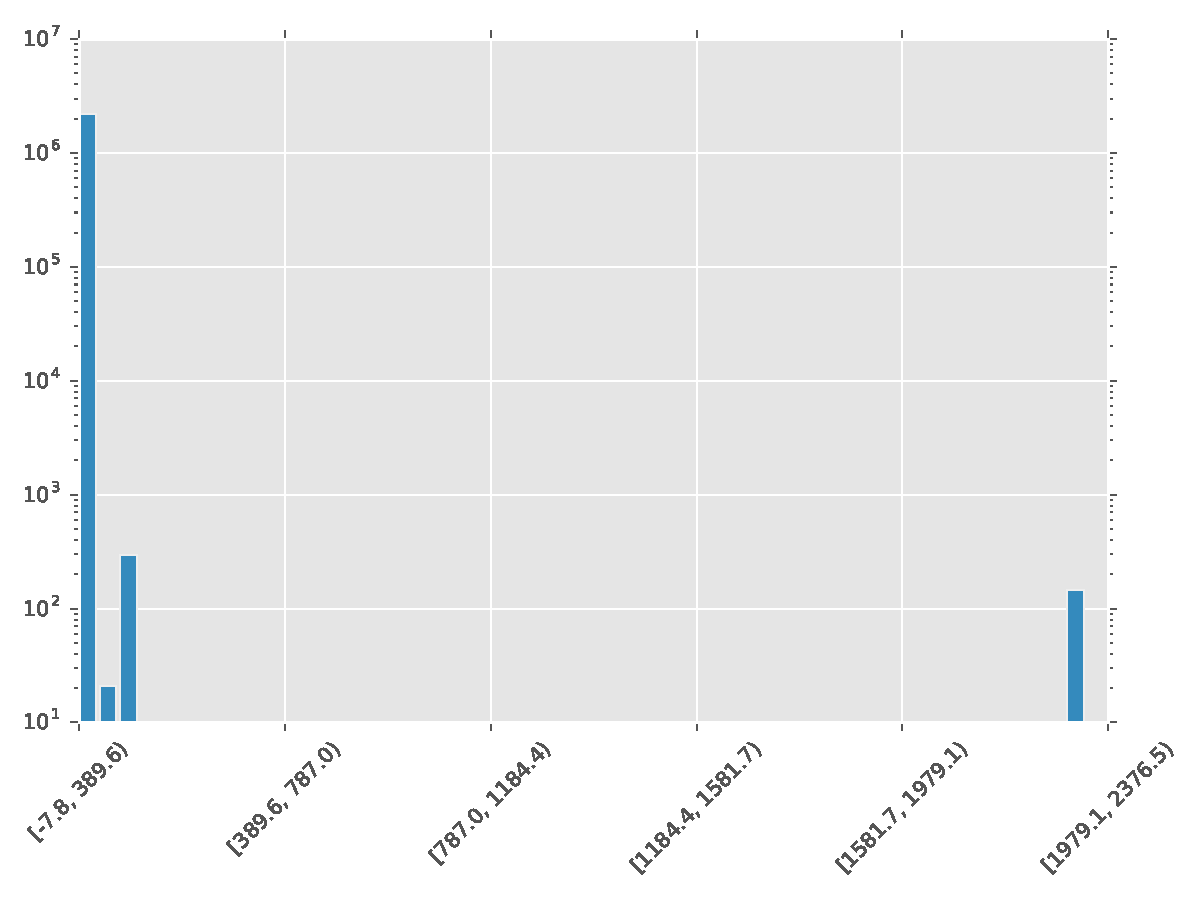
\includegraphics[width=\textwidth]{resources/histogramC}
        \caption{Histogram of weight values distribution.}
    \end{subfigure}%
    ~
    \begin{subfigure}[b]{0.32\textwidth}
        \centering
        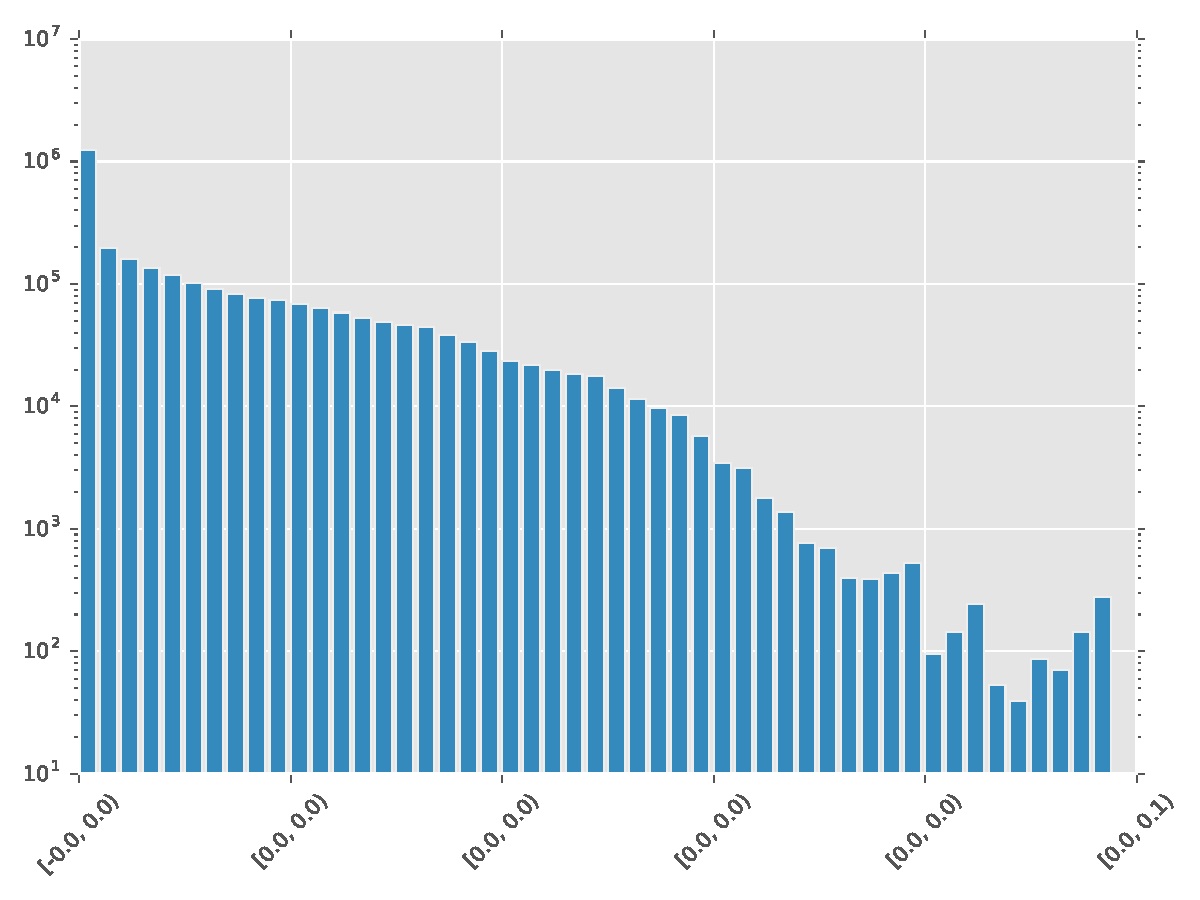
\includegraphics[width=\textwidth]{resources/histogramp}
        \caption{Histogram of pdf model values distribution.}
    \end{subfigure}
    ~
    \begin{subfigure}[b]{0.32\textwidth}
        \centering
        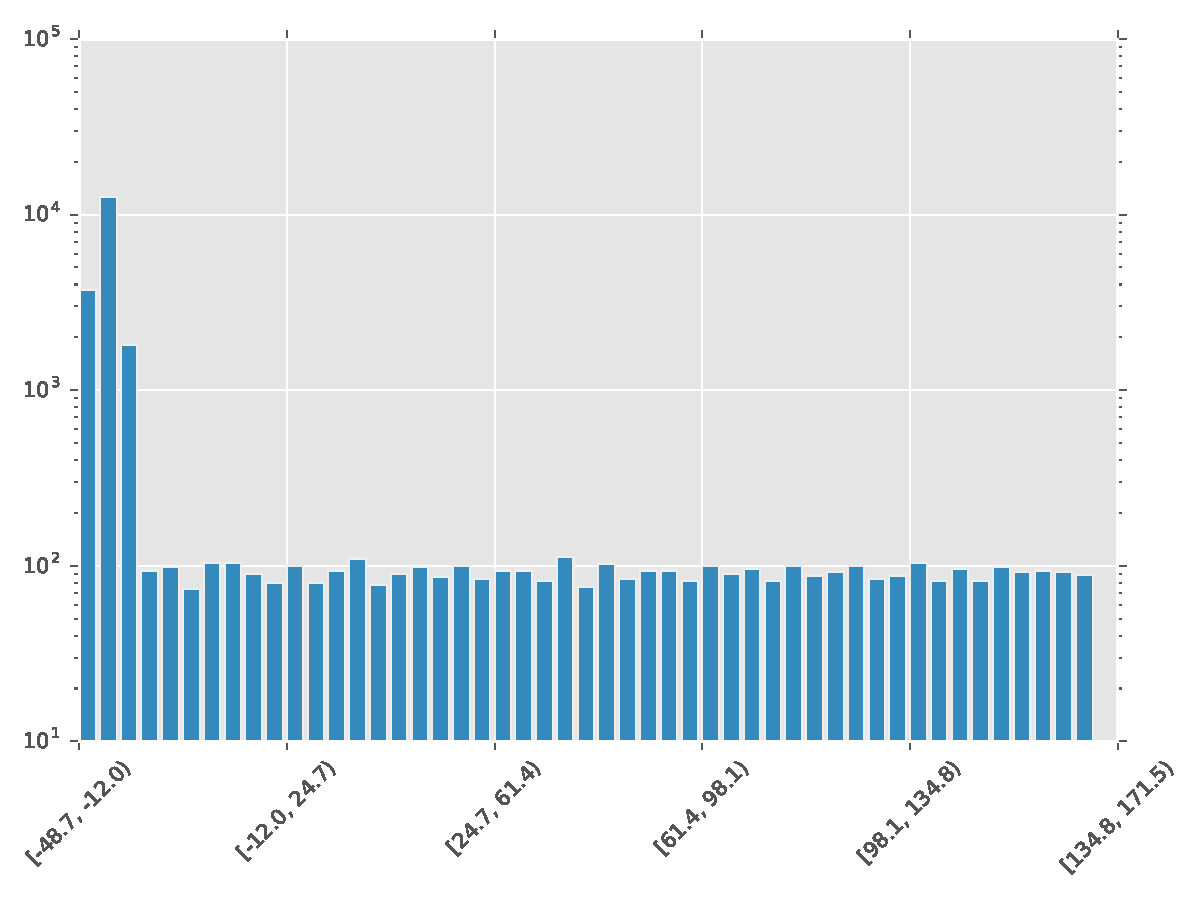
\includegraphics[width=\textwidth]{resources/histogramE}
        \caption{Histogram of E. kernel values distribution.}
    \end{subfigure}
    \caption{Value distributions made using \texttt{src/RunSystem/ProcessDynRangeFile.py}}
    \label{fig:value-distributions}
\end{figure}

\begin{table}[H]
    \centering
    \caption{The final ranges for the used \texttt{int16\_t} data representation.}
    \label{tab:final-ranges}
    \begin{tabular}{lll}
        \toprule
        \textbf{Value set} & \textbf{Range Min} & \textbf{Range Max} \\
        \midrule
        Weight      &  \num{-2048}  &  \num{2048}     \\
        PDF model   &  \num{-2}   &  \num{2}      \\
        Kernel      &  \num{-1/512} &  \num{1/512}    \\
        \bottomrule
    \end{tabular}
\end{table}

The speed-up that was measured with a fixed-point implementation based on the \texttt{int16\_t} type, and all values using the largest range (\num{2048}) was about \SIrange{31.5}{32}{\speedup} times kernel speed-up.
The next bottleneck is getting a faster conversion from the different ranges and a quick division that respects the fixed point nature of the values in the \texttt{int16\_t} datatype.
Instead of doing a normal integer division, one needs to shift the nominator to keep the results in the correct fixed-point format.
To implement fixed-point math properly the project would need parts of boost for the operator overloads to create a good class, so all the errors and other debugging issues go away.
But linking boost just for that is a step too far for this project.

Fixed point for NEON should also provide a speedup.
After some benchmarking we found that a 4 way f32 mult takes about \SI{9}{\cycles}, a 4 way 32 mult takes about \SI{5}{\cycles}, and 8 way 16 bit mult takes \SI{3}{\cycles}.
These cycle counts are from the measured time of millions of iterations and an assumed clock speed of \SI{740}{\mega\hertz}.

\end{document}